\chapter{How tos}\label{chap:how_tos}


\section{Some useful advice}
\begin{itemize}
	\item Use the asset folder for images
	\item Each chapter should be its own tex file
	\item If you have an image, reference it using the appropriate commands (see below)
	\item Each label should be created using this approach
	\begin{itemize}
		\item[] abbreviation:title
		\item[] where abbreviation $\in \{\text{prob,eq, fig, subfig, chap, sec, tab}\}$
	\end{itemize}
		\item Compile 2-3 times, sometimes one compilation might not be necessary to updated bibliography
	\item Use one bib file
	\item The bib entry should be preceded by a comment with a short description of what the paper is about. 
	\item To identify a paper, use this approach:
			\begin{itemize}
				\item[] firstAuthoutLastName + DateOfPublication + oneOrTwoWordsAboutThePaper
			\end{itemize}
	\item If you think about it makes sense to take a screenshot of the code to show it, think again
	\item If you have some algorithm you want to show, use the appropriate pseudo code instead of the code (see \algoref{algo:bofosort})
\end{itemize}




\section{How to reference stuff}\label{sec:general_definitions}
This is the best practice to reference stuff. For example, in order to refer to a definition, use \verb|\defref{def:positive_semidefinite}| (gives \defref{def:positive_semidefinite}) for each of the definitions. In this way, each reference is consistent. Similarly, the appropriate command shown in \tabref{tab:ref_commands}.

\begin{table}[h]
	\centering
	\begin{tabular}{|c|c|l|}
		\hline
		\texttt{\textbackslash secref\{YourLabel\}} & \secref{sec:general_definitions} &  \\ \hline
		\texttt{\textbackslash chapref\{YourLabel\}} & \chapref{chap:how_tos} &  \\ \hline
		\texttt{\textbackslash figref\{YourLabel\}} & \figref{fig:nyc_rn} &If using it with the label of a subfigure, \\&&includes the letter of subfigure as well.\\ \hline
		\texttt{\textbackslash equaref\{YourLabel\}} & \equaref{eq:equation_test} &  \\ \hline
		\texttt{\textbackslash problemref\{YourLabel\}} & \problemref{prob:example} &  \\ \hline
		\texttt{\textbackslash defref\{YourLabel\}} & \defref{def:positive_semidefinite} &  \\ \hline
		\texttt{\textbackslash exref\{YourLabel\}} & \exref{ex:example} &  \\ \hline
		\texttt{\textbackslash tabref\{YourLabel\}} &  \tabref{tab:ref_commands} & Chooses a specific figure, \\&&use only when it's clear to which \\&&figure you are talking about \\ \hline
		\texttt{\textbackslash subfigref\{YourLabel\}} & \subfigref{fig:nyc_simplified_roads} &  \\ \hline
		\texttt{\textbackslash appref\{YourLabel\}} & Appendix &  \\ \hline
	\end{tabular}
	\caption{Proposed reference commands}\label{tab:ref_commands}
\end{table}



\begin{problem}\label{prob:example} 
	Given a transportation network $\mathcal{G}$ and a set of vehicles $\mathcal{A}$, solve:
	\begin{align}
		\text{min}& 
		\mathcal{J}_T = \sum_{a \in \mathcal{A}} \sum_{(u, v) \in \mathcal{E}} T^a_{ u,v} V^a_{u,v}
		\nonumber\\
		\text{s.t.} &\nonumber\\
		&\sum_{u \in \mathcal{V}} V^a_{u, v} - \sum_{w \in \mathcal{V}} V^a_{v, w} = 0 \quad \forall a \in \mathcal{A}, v \in \mathcal{V} \setminus \{\underline{s_a}, \bar{t_a}\} \label{eq:flow_conservation_graph_u} \\
		&\sum_{ u \in \mathcal{N}^+_{\underline{s_a}} }V^a_{ \underline{s_a},u} = 1 \quad \forall a \in \mathcal{A} \label{eq:flow_cons_arrival_graph_u}\\
		&\sum_{u \in \mathcal{N}^-_{\bar{t_a}} } V^a_{u, \bar{t_a}} = 1 \quad \forall a \in \mathcal{A} \label{eq:flow_cons_departure_graph_u}\\
		\nonumber
	\end{align}
\end{problem}

\begin{definition}\label{def:positive_semidefinite}
	A symmetric matrix $A$ is said to be positive semidefinite if, for any non-zero column vector $x$, the following inequality holds:
	\begin{equation}
		x^T Ax \geq 0\label{eq:equation_test}
	\end{equation}
	Here, $x^T$ represents the transpose of the vector $x$, and $x^T Ax$ is the quadratic form associated with the matrix $A$. Another way to express positive semidefiniteness is in terms of eigenvalues. A symmetric matrix $A$ is positive semidefinite if and only if all of its eigenvalues are non-negative.\\
	Mathematically, $A \succeq 0 $ indicates positive semidefiniteness.
\end{definition}

\begin{example}\label{ex:example}
	This is an example
\end{example}


\begin{figure}[tbh]
	\centering
	\begin{subfigure}[b]{0.32\textwidth}
		\centering
		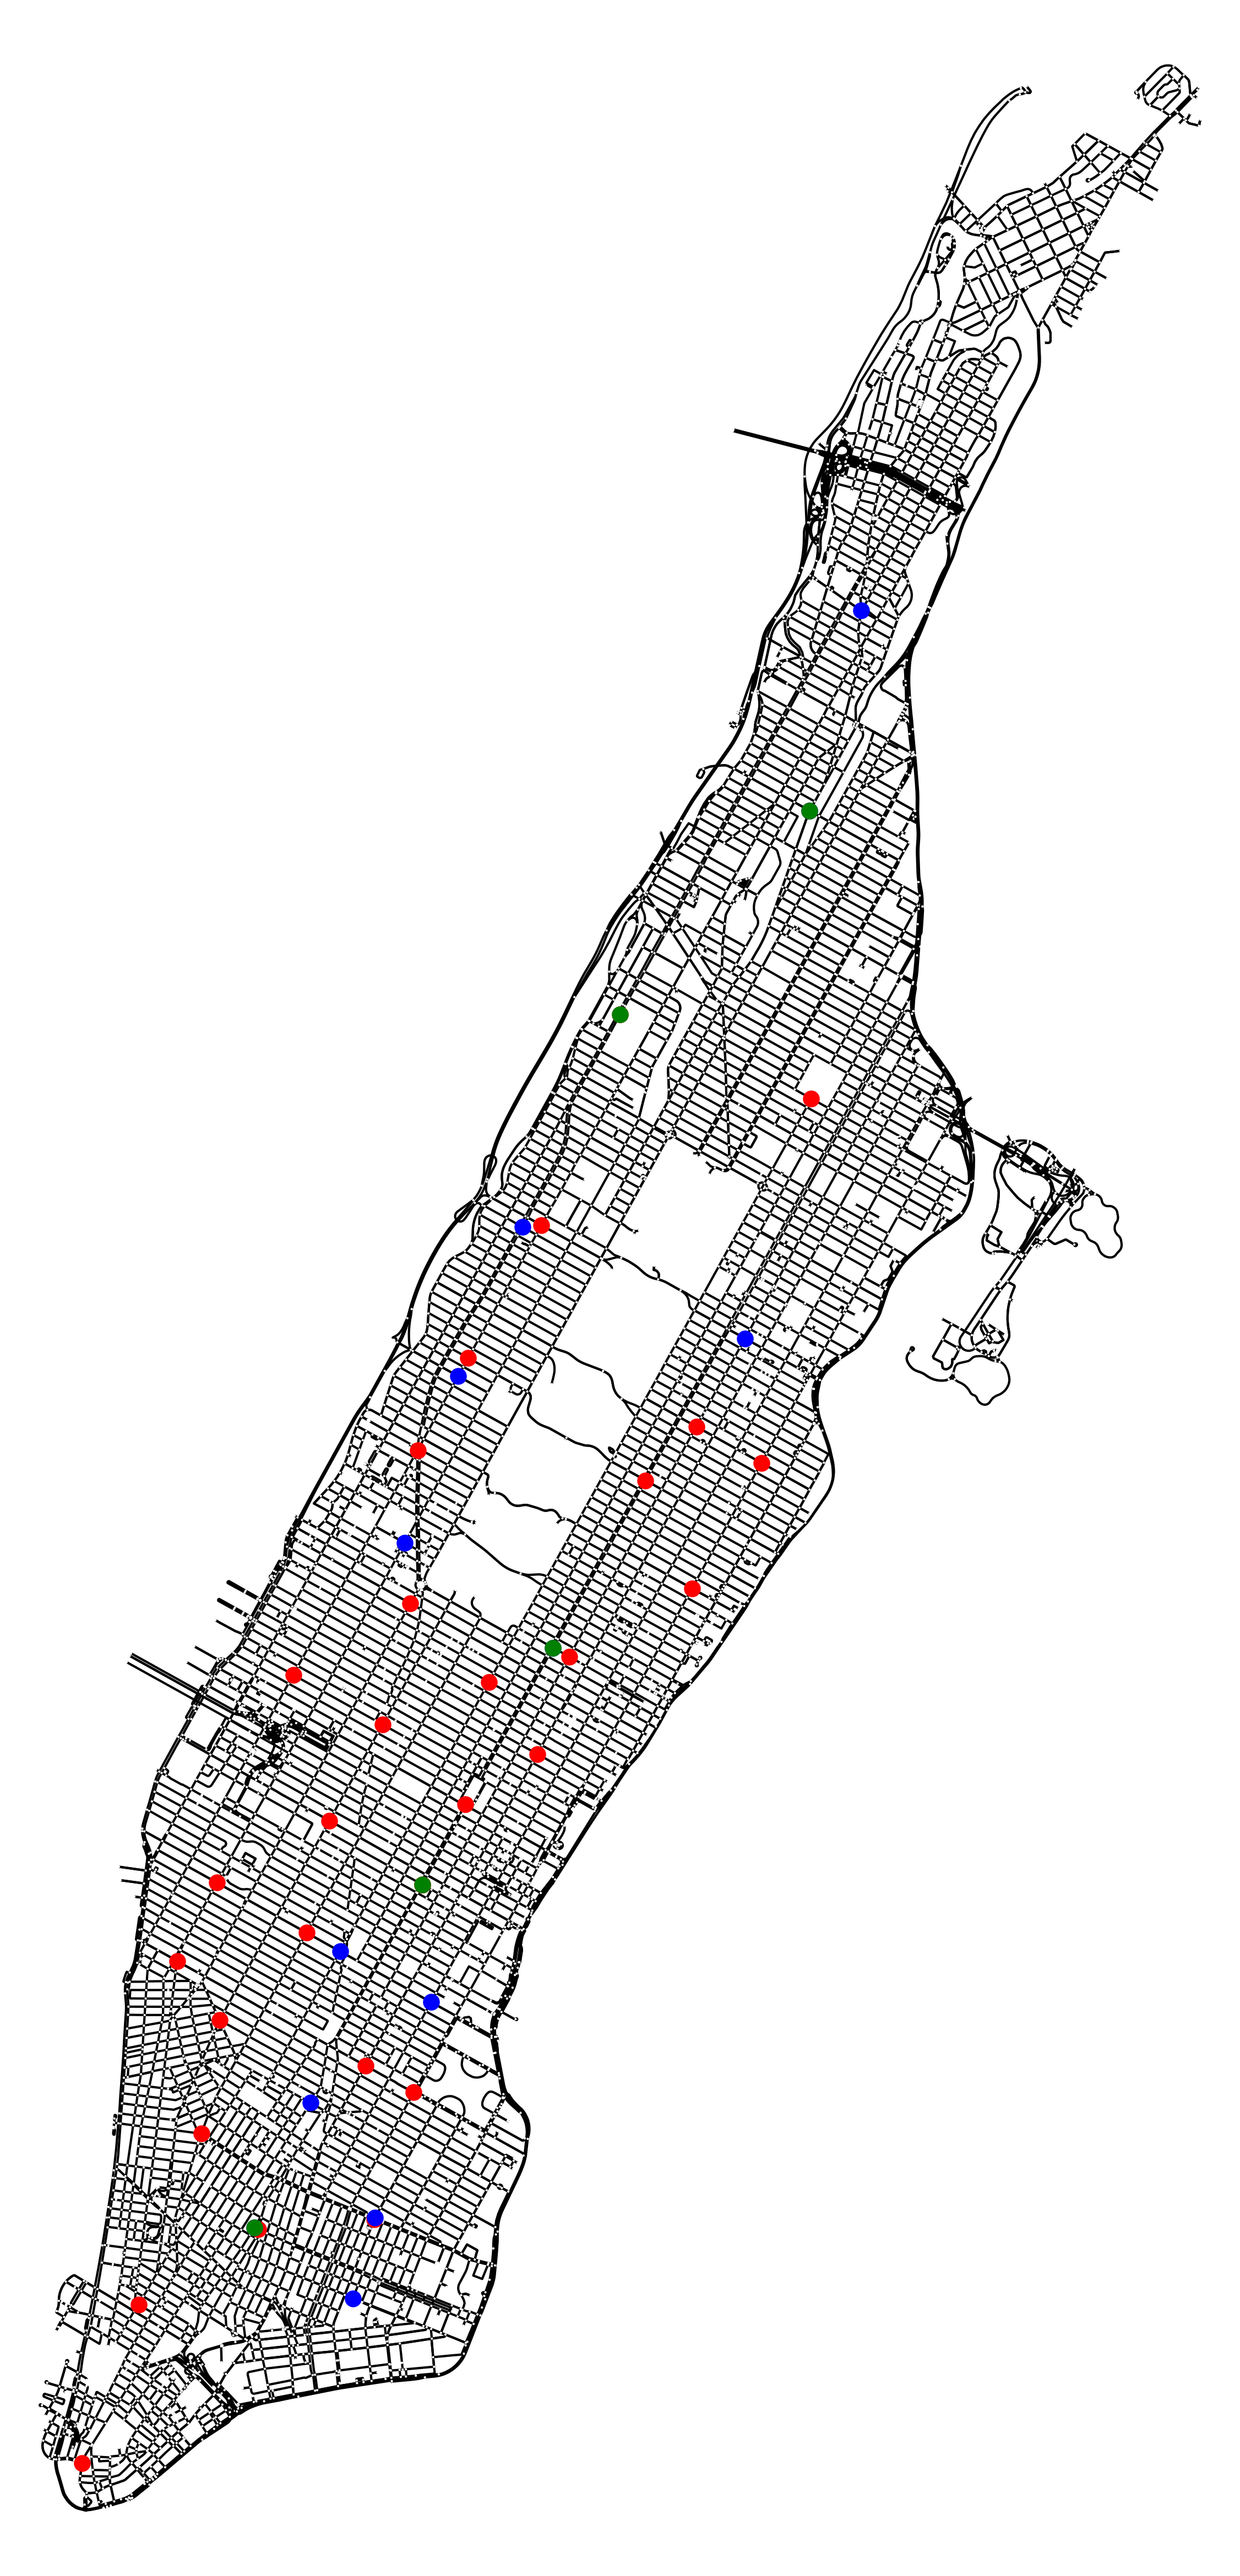
\includegraphics[width=\textwidth]{assets/img/new_york_vanilla_info.png}
		\caption{}
		\label{fig:nyc_rn_info}
	\end{subfigure}
	\begin{subfigure}[b]{0.32\textwidth}
		\centering
		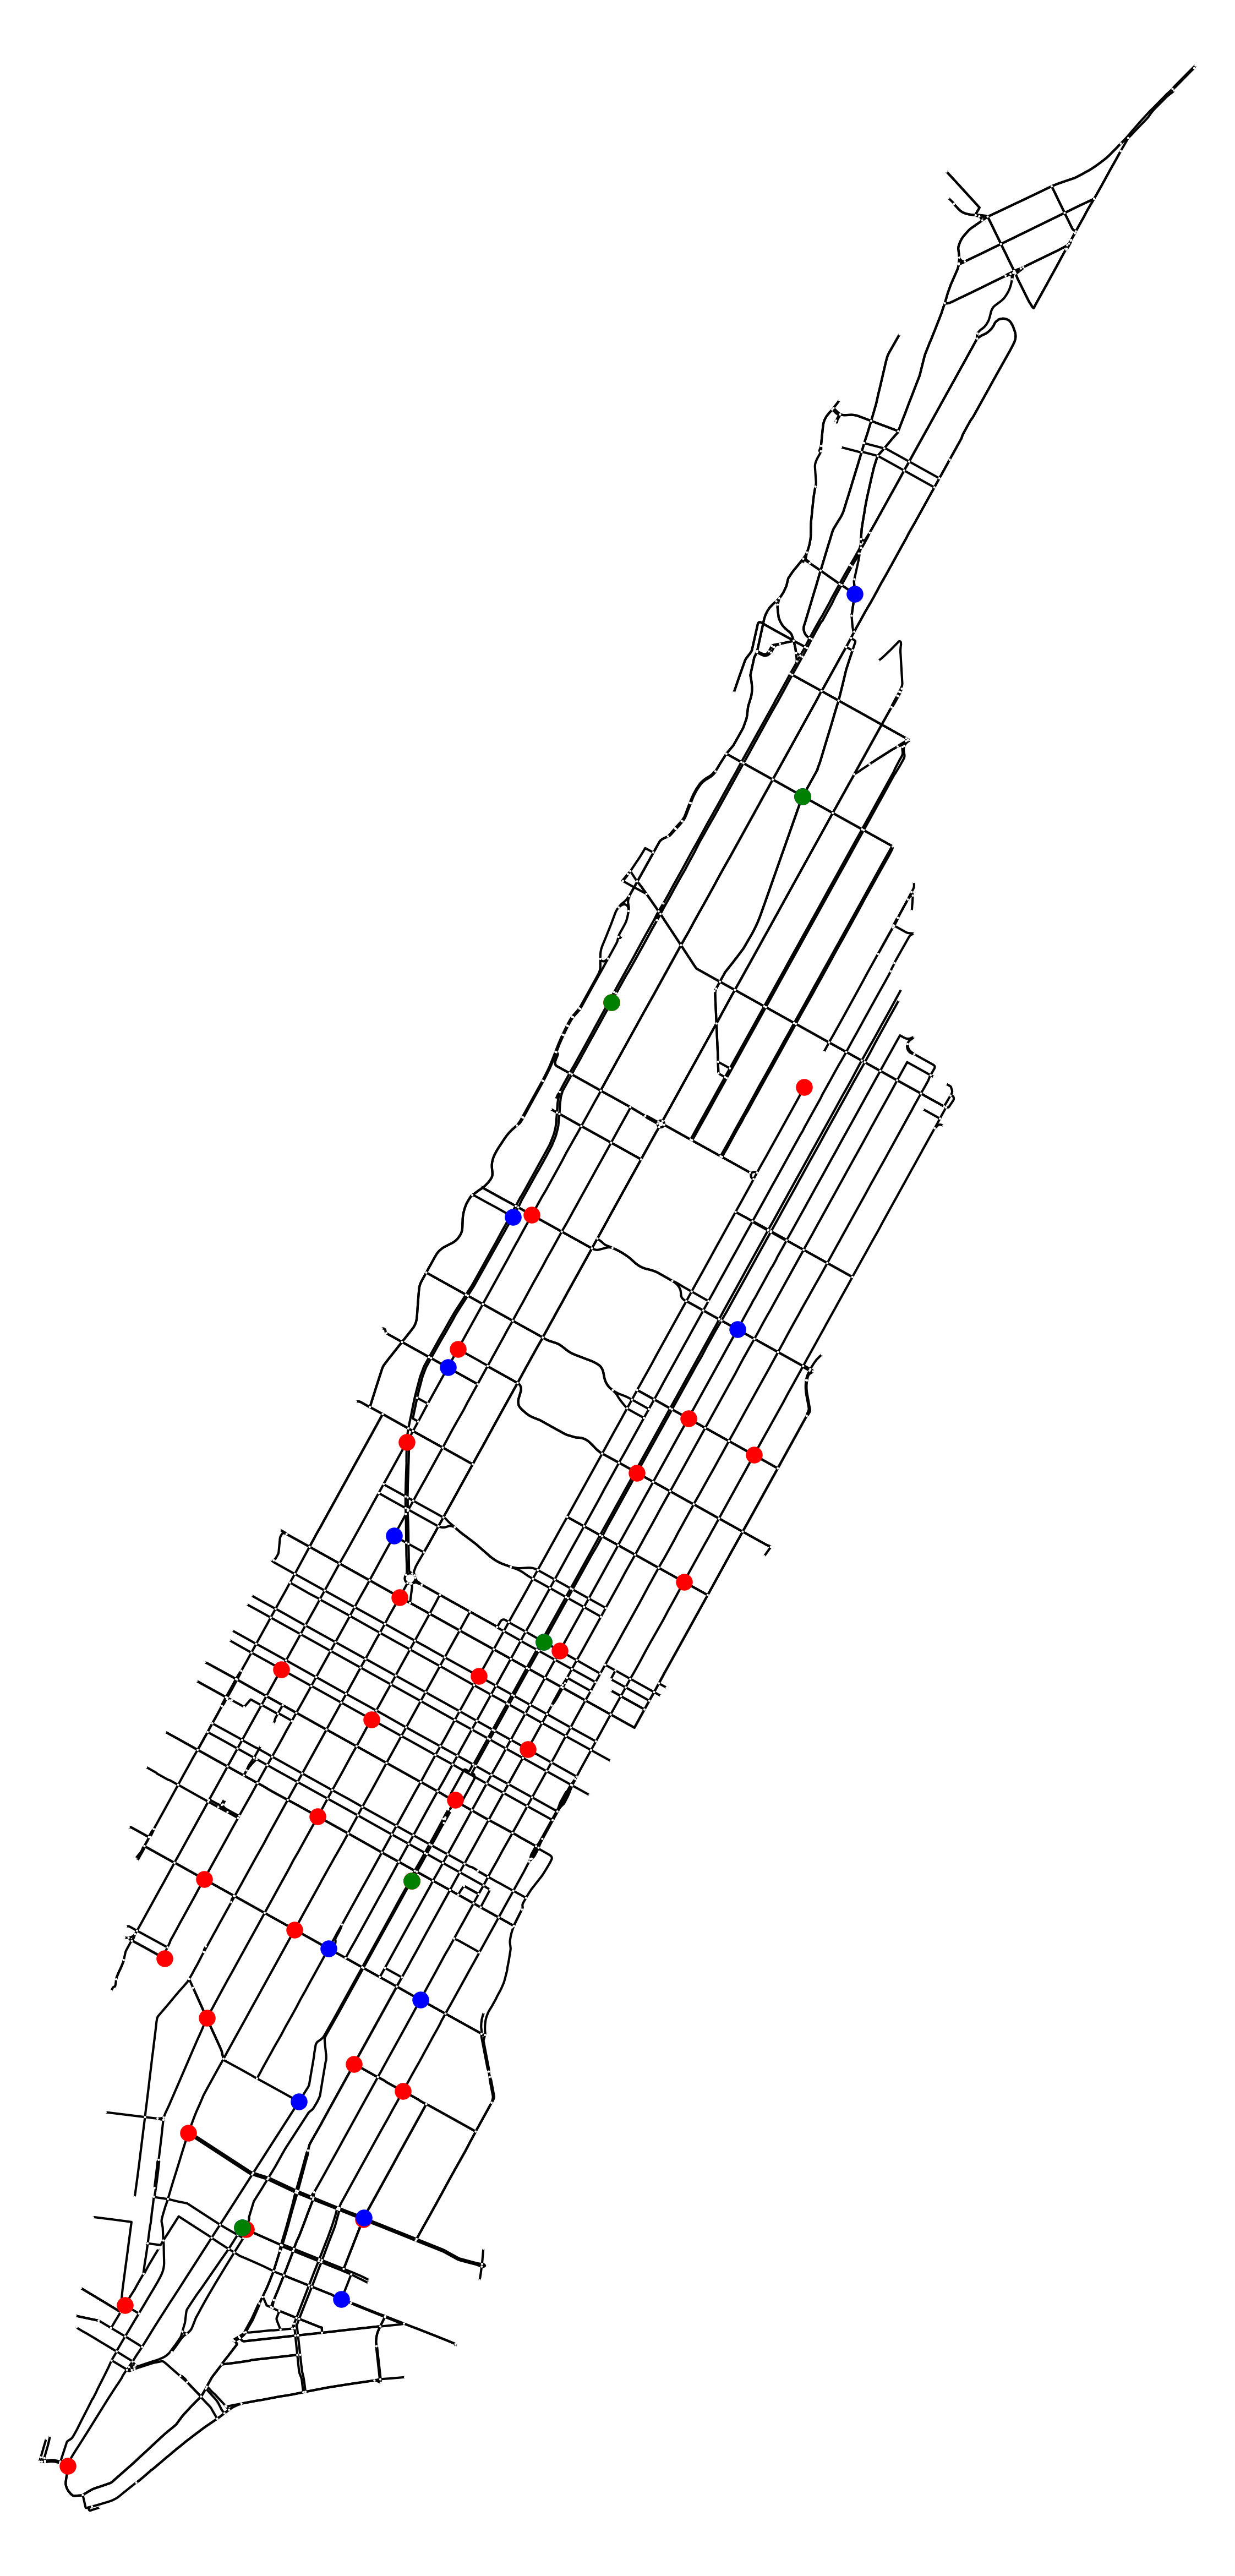
\includegraphics[width=\textwidth]{assets/img/new_york_simplified_info.png}
		\caption{}
		\label{fig:nyc_simplified_info}
	\end{subfigure}
	\begin{subfigure}[b]{0.32\textwidth}
		\centering
		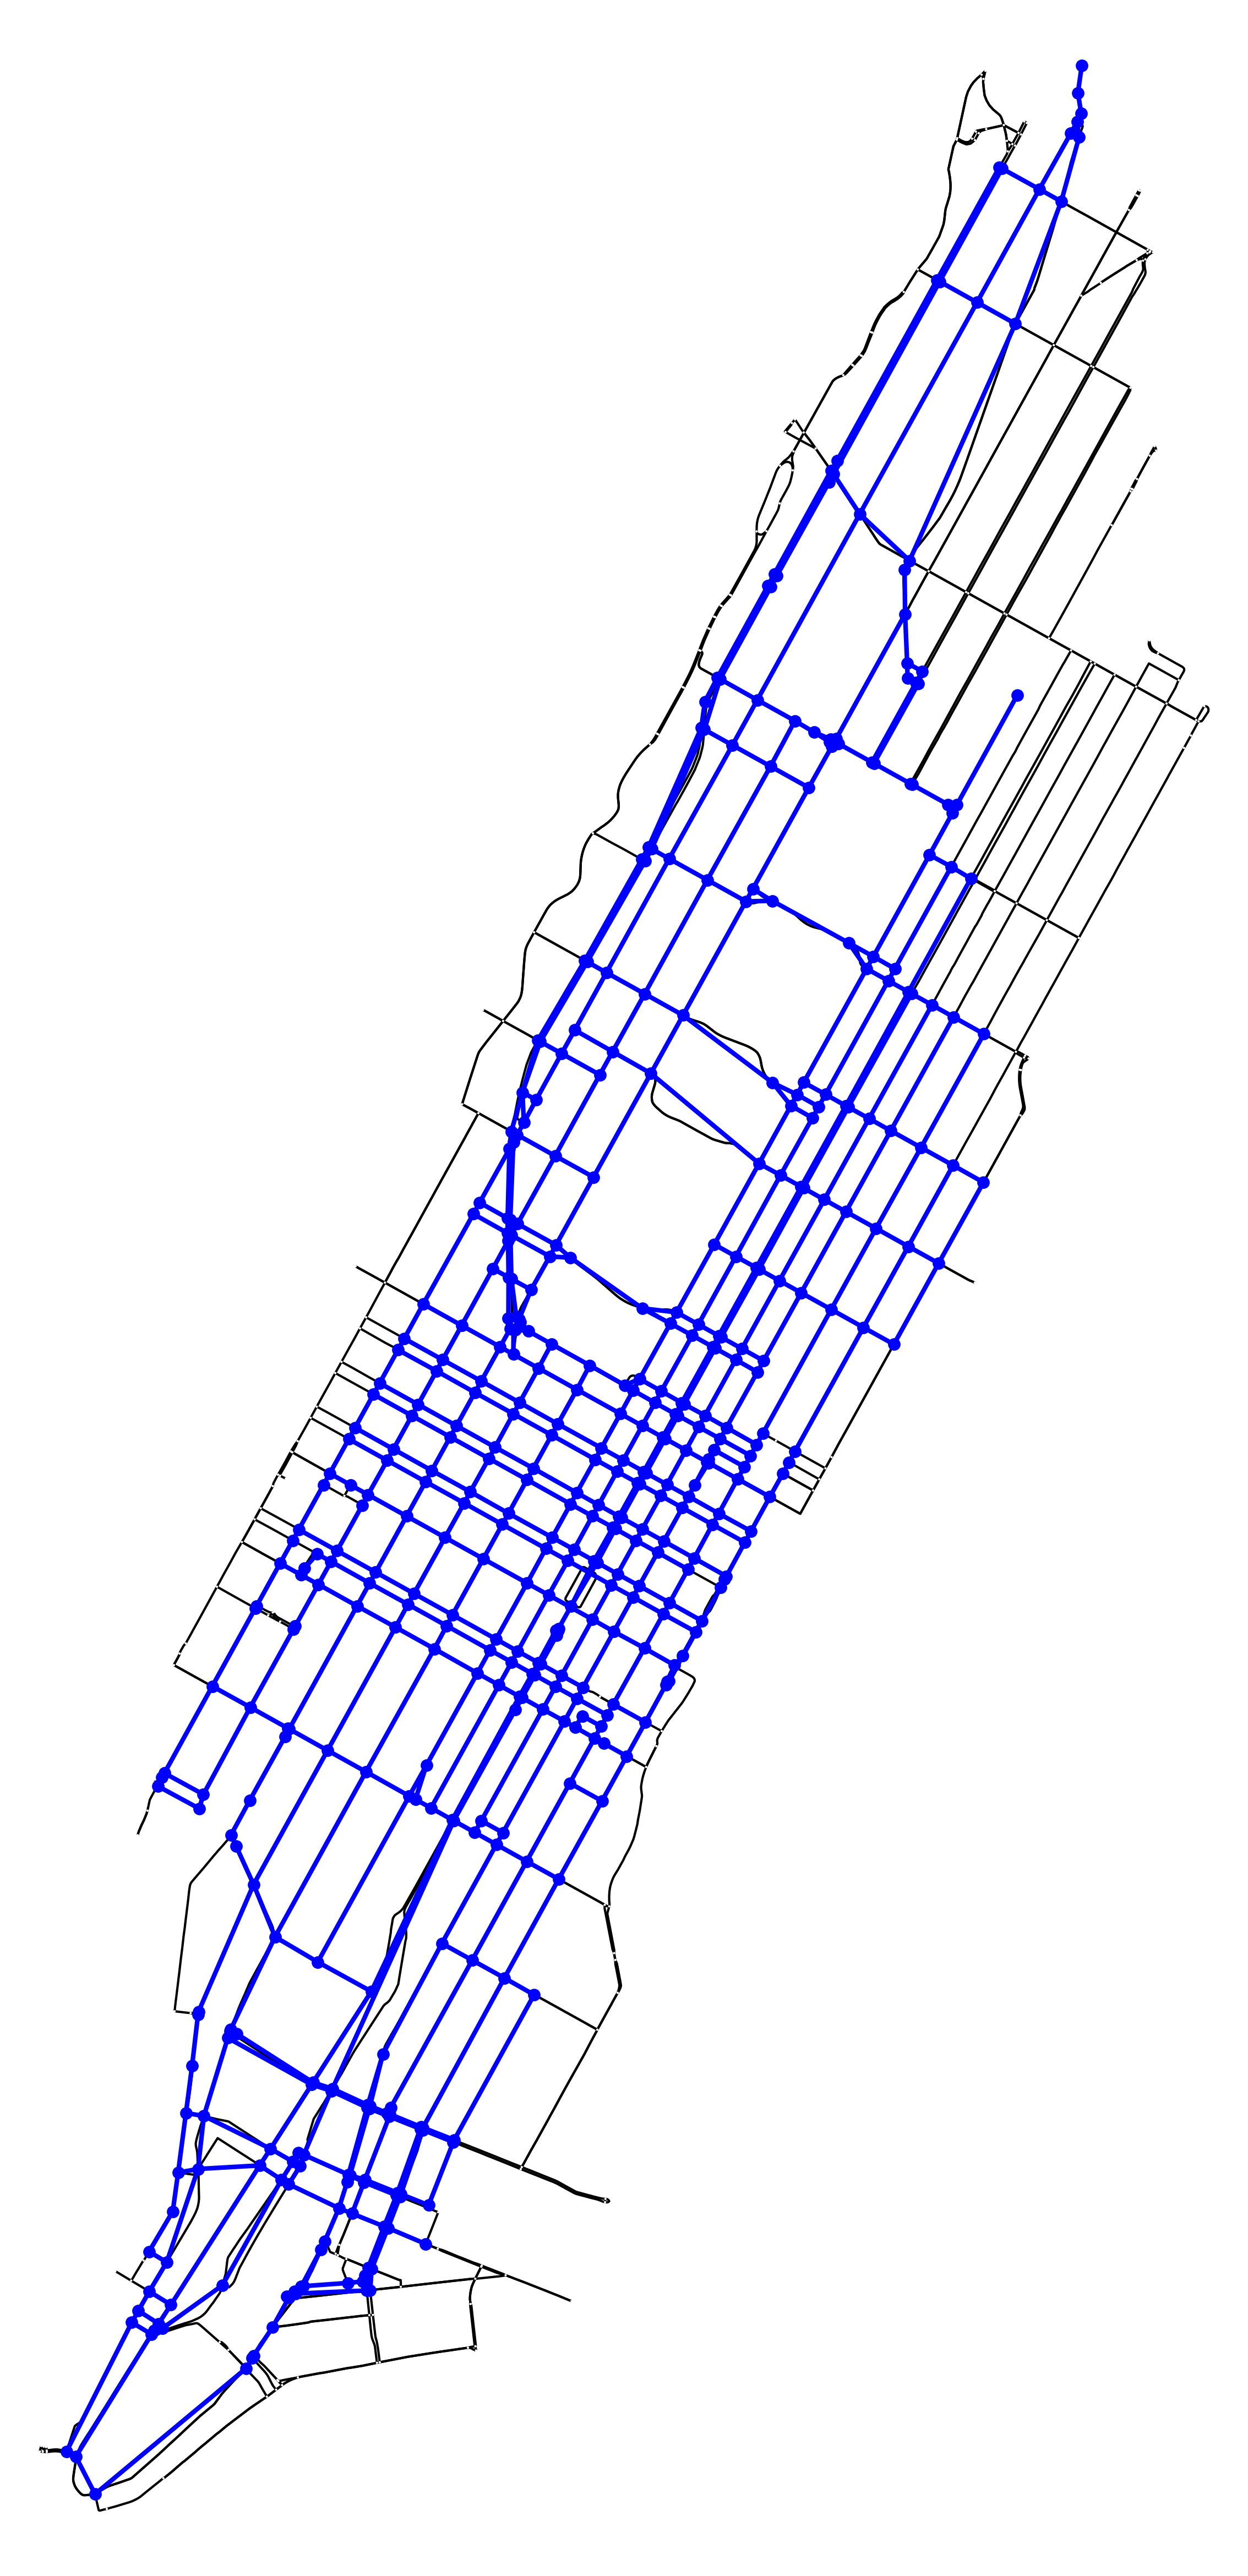
\includegraphics[width=\textwidth]{assets/img/new_york_simplified_roads.png}
		\caption{}
		\label{fig:nyc_simplified_roads}
	\end{subfigure}
	
	\caption[Title In the TOC]{Description }
	\label{fig:nyc_rn}
\end{figure}


\begin{figure}
	\begin{tikzpicture}
		\begin{umlpackage}{p} % package-p
			\begin{umlpackage}{sp1} % package-sp1
				\umlclass[ class]{A}{ % class-A
					n : uint \\
					t : float
				}{}
				\umlclass[class,y=-3]{B}{ % class-B
					d : double
				}{
					\umlvirt{setB(b : B) : void} \\
					getB() : B
				}
			\end{umlpackage}
			\begin{umlpackage}[x=10,y=-6]{sp2} % package-sp2
				\umlinterface[class]{C}{ % class-C
					n : uint \\
					s : string
				}{}
			\end{umlpackage}
			\umlclass[class, x=2,y=-10]{D}{ % class-D
				n : uint
			}{}
		\end{umlpackage}
		
		\umlassoc[geometry=-|-, arg1=tata, mult1=*, pos1=0.3, arg2=toto, mult2=1, pos2=2.9, align2=left]{C}{B}
		\umlunicompo[geometry=-|, arg=titi, mult=*, pos=1.7, stereo=vector]{D}{C}
		\umlimport[geometry=|-, anchors=90 and 50, name=import]{sp2}{sp1}
		\umlaggreg[arg=tutu, mult=1, pos=0.8, angle1=30, angle2=60, loopsize=2cm]{D}{D}
		\umlinherit[geometry=-|]{D}{B}
		\umlnote[x=2.5,y=-6, width=3.5cm]{B}{
			\footnotesize{I am a note that belongs to class B.}
		}
		\umlnote[x=7.5,y=-1.5]{import-2}{
			\footnotesize{I am a note that concerns the import relationship.}
		}
		
	\end{tikzpicture}
	\caption{Example of a UML class diagram}
\end{figure}


\begin{figure}
\begin{tikzpicture}
	
	\begin{umlsystem}[x=4]{The system}
		\umlusecase{use case 1} % usecase-1
		\umlusecase[y=-2]{use case 2} % usecase-2
		\umlusecase[y=-4]{use case 3} % usecase-3
		\umlusecase[x=4, y=-2, width=1.5cm]{ % usecase-4
			\shortstack{use case 4\\\footnotesize{on 2 lines}}
		}
		\umlusecase[x=6]{use case 5} % usecase-5
		\umlusecase[x=6, y=-4]{use case 6} % usecase-6
	\end{umlsystem}
	
	\umlactor{user}
	\umlactor[y=-3]{subuser}
	\umlactor[x=14, y=-1.5]{admin}
	
	\umlinherit{subuser}{user}
	\umlassoc{user}{usecase-1}
	\umlassoc{subuser}{usecase-2}
	\umlassoc{subuser}{usecase-3}
	\umlassoc{admin}{usecase-5}
	\umlassoc{admin}{usecase-6}
	\umlinherit{usecase-2}{usecase-1}
	\umlVHextend{usecase-5}{usecase-4}
	\umlinclude[name=incl]{usecase-3}{usecase-4}
	
	\umlnote[x=7, y=-7]{incl-1}{
		\footnotesize{note on include dependency}
	}
	
\end{tikzpicture}
\caption{Example of Use case diagram}
\end{figure}
\begin{figure}
\begin{tikzpicture}[scale=.85]
	
	\begin{umlseqdiag}
		\umlactor[class=A]{a}
		\umldatabase[class=B, fill=blue!20]{b}
		\umlmulti[class=C]{c}
		\umlobject[class=D]{d}
		\begin{umlcall}[op=opa(), type=synchron, return=0]{a}{b}
			\begin{umlfragment}
				\begin{umlcall}[op=opb(), type=synchron, return=1]{b}{c}
					\begin{umlfragment}[type=alt, label=condition, inner xsep=8, fill=green!10]
						\begin{umlcall}[op=opc(), type=asynchron, fill=red!10]{c}{d}
						\end{umlcall}
						\begin{umlcall}[type=return]{c}{b}
						\end{umlcall}
						\umlfpart[default]
						\begin{umlcall}[op=opd(), type=synchron, return=3]{c}{d}
						\end{umlcall}
					\end{umlfragment}
				\end{umlcall}
			\end{umlfragment}
			\begin{umlfragment}
				\begin{umlcallself}[op=ope(), type=synchron, return=4]{b}
					\begin{umlfragment}[type=assert]
						\begin{umlcall}[op=opf(), type=synchron, return=5]{b}{c}
						\end{umlcall}
					\end{umlfragment}
				\end{umlcallself}
			\end{umlfragment}
		\end{umlcall}
		\umlcreatecall[class=E,x=8]{a}{e}
		\begin{umlfragment}
			\begin{umlcall}[op=opg(), name=test, type=synchron, return=6, dt=7, fill=red!10]{a}{e}
				\umlcreatecall[class=F, stereo=boundary, x=12]{e}{f}
			\end{umlcall}
			\begin{umlcall}[op=oph(), type=synchron, return=7]{a}{e}
			\end{umlcall}
		\end{umlfragment}
	\end{umlseqdiag}
	
\end{tikzpicture}
\end{figure}


\begin{algorithm}
	\caption{BogoSort}\label{algo:bofosort}
	\begin{algorithmic}
		\Function{BogoSort}{$A$}
		\While{not \Call{IsSorted}{$A$}}
		\State \Call{Shuffle}{$A$}
		\EndWhile
		\EndFunction
	\end{algorithmic}
\end{algorithm}

